\documentclass{report}
\usepackage{homework}
\usepackage{url}
\solstrue

\usepackage{graphicx}
\graphicspath{{figures/}}

\renewcommand{\hmwkTitle}{Homework 6}

\begin{document}
\mktitle

\begin{problem}
Suppose an application generates chunks of 60 bytes of data, each chunk gets encapsulated in a TCP segment, and then an IP datagram.

\begin{enumerate}
\item What percentage of each datagram will be overhead, and what percentage will be application data?

\item What would be the overhead if each TCP segment include 100 of application chunks (i.e., $100 \times 60$ bytes), assuming the maximum size of an IP packet is 500 bytes and sending such big TCP payload would require fragmentation.
\end{enumerate}

\begin{answer}{40em}
    Write your answer here
\end{answer}

\end{problem}



\newpage



\begin{problem}

Consider the router trying to send the following IP packet:

\begin{figure}[!h]
\center
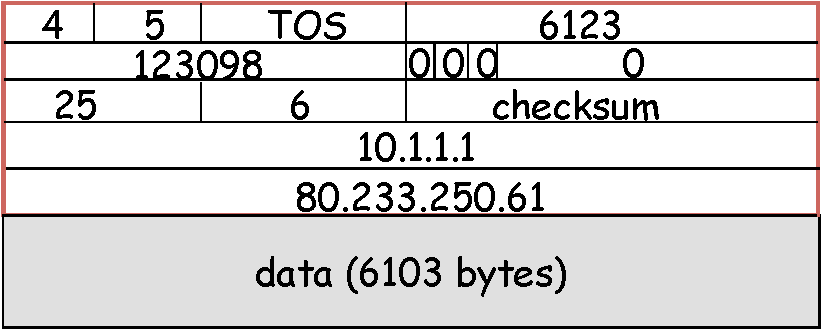
\includegraphics[scale=0.8]{hw6-frag.pdf}
\caption{An IP packet.}
\label{fig:ip-frag}
\end{figure}

Assuming that the maximum transmission unit that can be transferred over the link is 1400 bytes.
For each of the fragment show the header length, total length, identification, flags, fragment offset, TTL, protocol fields, and IP payload size.



\begin{answer}{35em}
  Write your answer using the table below\\
  
  \begin{tabular}[h]{|c|c|c|c|c|c|c|c|}
  \hline
  Header length &
  Total length &
  Identification &
  Flags &
  Fragment offset &
  TTL &
  Protocol &
  Data size \\
  \hline
  & & & & & & & \\
  & & & & & & & \\
  & & & & & & & \\
  & & & & & & & \\
  & & & & & & & \\
  & & & & & & & \\
  & & & & & & & \\
  & & & & & & & \\
  & & & & & & & \\
  & & & & & & & \\
  & & & & & & & \\
  & & & & & & & \\
  & & & & & & & \\
  & & & & & & & \\
  & & & & & & & \\
  & & & & & & & \\
  & & & & & & & \\
  & & & & & & & \\
  & & & & & & & \\
  & & & & & & & \\
  & & & & & & & \\
  & & & & & & & \\
  \hline
\end{tabular}

\end{answer}

\end{problem}


\newpage



\begin{problem}
Calculate the network mask, the number of bits of the network, the number of endpoint addresses in the network (excluding special addresses), the network address, and the broadcast address of the network for the following:

\begin{enumerate}
\item 131.179.196.0/24
\item 169.232.34.48/30
\item 196.22.136.0/21
\item 93.181.192.0, netmask 255.255.224.0
\item 10.128.0.0, netmask 255.192.0.0
\end{enumerate}



\begin{answer}{35em}
  Write your answer here
\end{answer}

\end{problem}

\newpage



\begin{problem}
Why is the IP header checksum recalculated at every router?

\begin{answer}{40em}
    Write your answer here
\end{answer}

\end{problem}

\newpage



\begin{problem}
Install \textit{Wireshark} (\url{https://www.wireshark.org/}). Then, (i) start capturing a packet trace from your network interface, (ii) open a web browser, (iii) go to \url{https://www.cs.ucla.edu/}, (iv) and then stop capturing the trace.

Investigate any TCP packet from your network interface to the UCLA CS web server.
What is the IP address of your network interface? What is the IP address of www.cs.ucla.edu? Provide the screenshot that shows the IP addresses in the investigated packet.

\begin{answer}{40em}
    Write your answer here (Also, attach the screenshot)
\end{answer}

\end{problem}

\end{document}
